\documentclass[aspectratio=169]{beamer}

\usepackage{ulem}
\usepackage{dejavu}
\usepackage{listings}
\usepackage{hyperref}

\mode<presentation>{
  \usetheme{Rochester}
}
\beamertemplatenavigationsymbolsempty
\usecolortheme[RGB={115,79,150}]{structure}
%\usefonttheme{structurebold}

% https://tex.stackexchange.com/questions/44983/beamer-removing-headline-and-its-space-on-a-single-frame-for-plan-but-keepin
\makeatletter
    \newenvironment{withoutheadline}{
        \setbeamertemplate{headline}[default]
        \def\beamer@entrycode{\vspace*{-\headheight}}
    }{}
\makeatother


\title{Introducing the Fortran-lang community}
\institute{
\includegraphics[width=0.5in]{fortran_logo_256x256}}
\author{\small Ivan Pribec 
  \and Vincent Magnin
  \and Asdrubal Lozada-Blanco
  \and Ond\v{r}ej \v{C}ertik
  \and Jeremie Vandenplas
  \and Milan Curcic
  \and Rohit Goswami
  \and Sebastian Ehlert 
  \and Ioannis Nikiteas
  \and Gabriele Bellomia
  \and Carl Burkert
  \and Emanuele Pagone
\and Brad Richardson \and Amir Shahmoradi}
\date{\footnotesize deRSE23 - 20-22 Feb 2023, Paderborn\\
Conference for Research Software Engineering in Germany}

\begin{document}

\begin{frame}
  \titlepage
\end{frame}

\begin{frame}
  \frametitle{Overview}

\begin{block}{Why Fortran?}
	\begin{itemize}
		\item 60+ years of high-level, high-performance computing
	\end{itemize}
\end{block}

\begin{block}{Fortran-lang community}
	\begin{itemize}
		\item State of the Fortran ecosystem
		\item A new online community for Fortran users
            \item Fortran-lang open source software 
	\end{itemize}
\end{block}

\begin{block}{The future is bright}
	\begin{itemize}
		\item Current projects
	\end{itemize}
\end{block}

\end{frame}

\begin{frame}
\frametitle{Fortran Summary}

\begin{itemize}
\item Developed in 1954-1957 at IBM (over 60 years old).
\item Name stands for \textit{FOR}mula \textit{TRAN}slation.
\item The purpose was (and remains) translation of mathematical formulae to machine code for scientists and engineers.
\item First high-level, cross-platform programming language; highly influential.
\item Many scientific apps and libraries developed in Fortran.
\item Base language has evolved, current standard ISO/IEC 1539-1:2018.
\item Supports multiple programming paradigms: procedural, object-oriented, functional, parallel
\end{itemize}
\end{frame}

\begin{frame}
\frametitle{Relevance of Fortran for Science}
\begin{columns}[T] % align columns
\begin{column}{.38\textwidth}
\centering
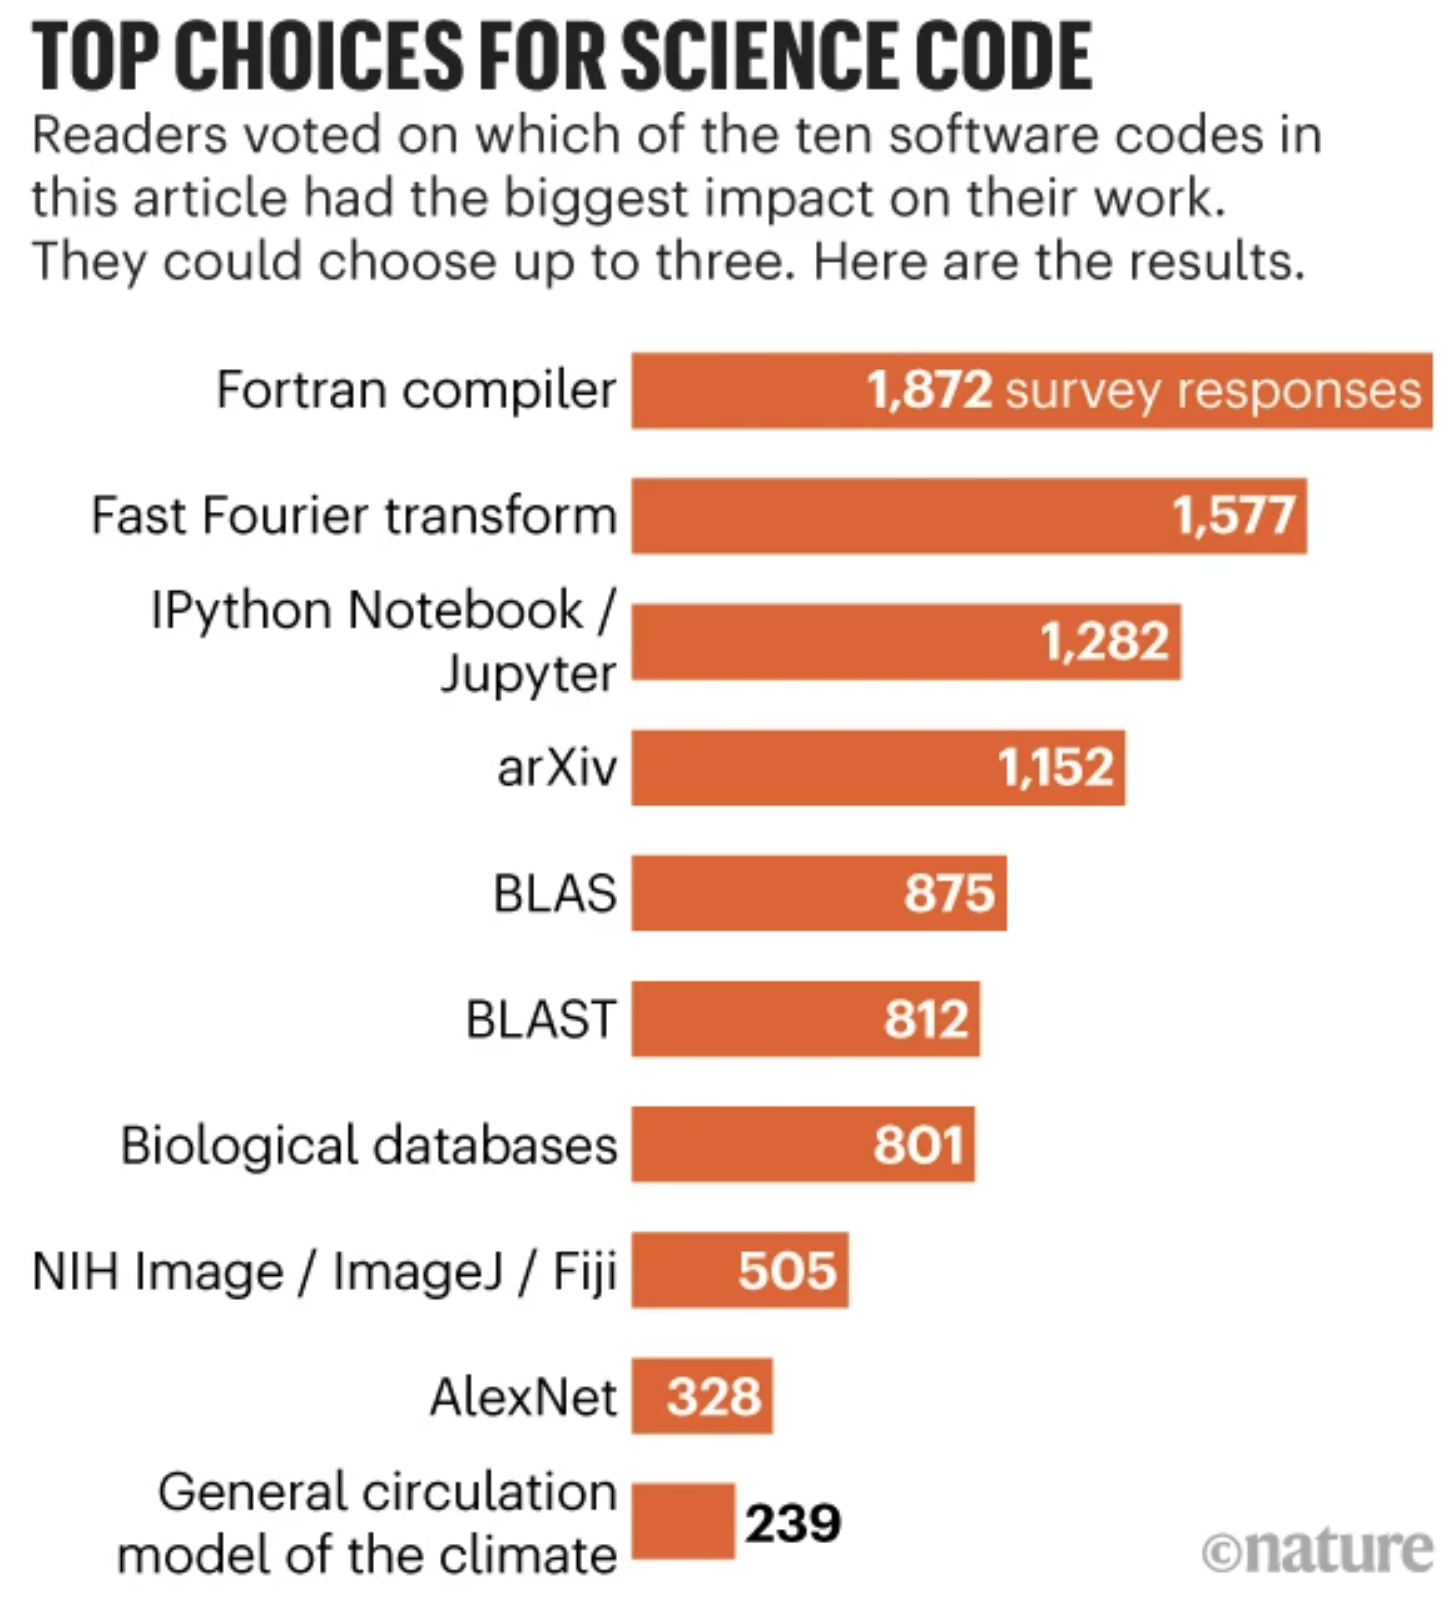
\includegraphics[width=0.9\textwidth]{nature_screenshot}
\begin{itemize}
    \item \footnotesize Ten computer codes that transformed science, \textit{Nature} 589, 344-348 (2021)
\end{itemize}
\end{column}%
\hfill%
\begin{column}{.6\textwidth}

    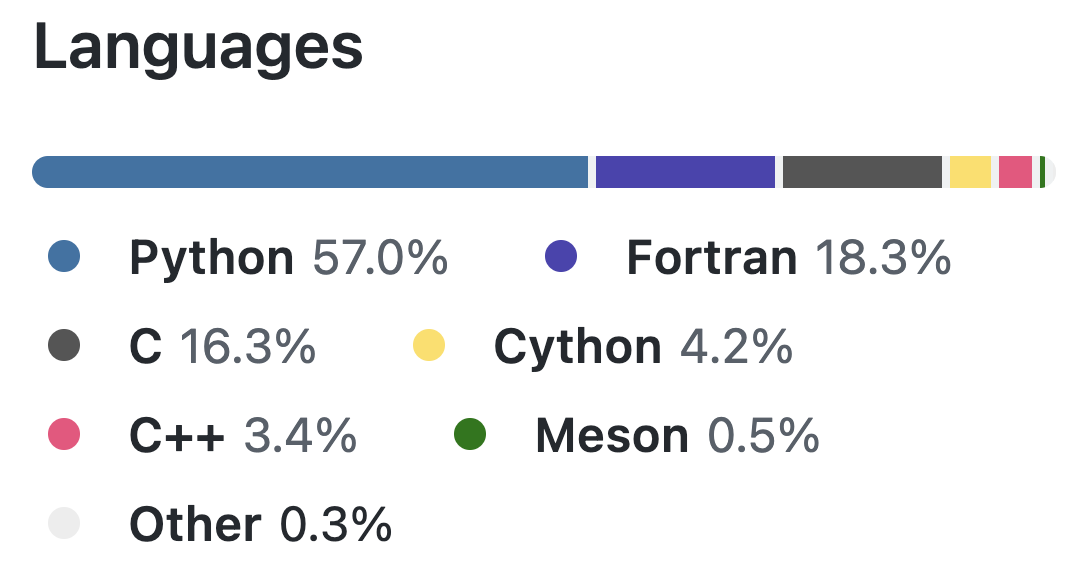
\includegraphics[width=0.58\textwidth]{scipy_screenshot.png}
\begin{itemize}
    \item \footnotesize SciPy (\url{https://github.com/scipy/scipy})
\end{itemize}
\vspace{0.1in}
    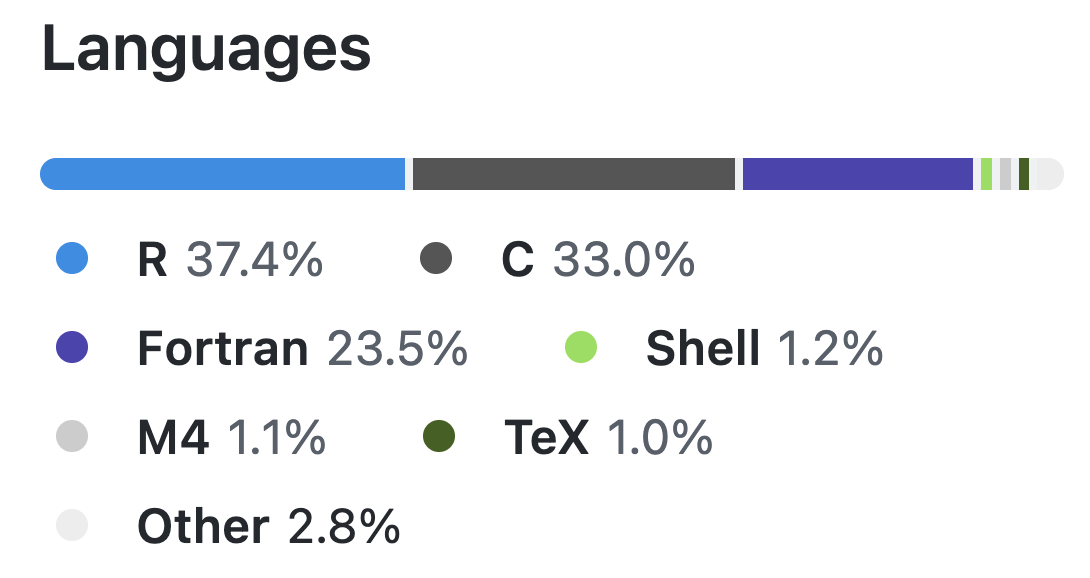
\includegraphics[width=0.58\textwidth]{r-source_screenshot.png}
\begin{itemize}
    \item \footnotesize R (\url{https://github.com/wch/r-source})
\end{itemize}
\end{column}%
\end{columns}

\end{frame}

\begin{frame}{Some wisdoms from the past}
\begin{block}{}
  {``FORTRAN has for most of [its] life been the blue-collar worker of the programming language set. What it lacked in [\textit{savoir faire}] and style, it returned in cost effectiveness.''}
  \vskip1mm
  \hspace*\fill{\small--- Martin N. Greenfield}
\end{block}

{\scriptsize Source: Greenfield, Martin N. ``History of FORTRAN standardization.'' Proceedings of the June 7-10, 1982, National Computer Conference. 1982.}

\begin{block}{}
  {``FORTRAN is a language to avoid---unless you want some answers.''}
  \vskip1mm
  \hspace*\fill{\small--- Anonymous}
\end{block}

{\scriptsize Source: Mark Jones Lorenzo, The History of the Fortran Programming Language, 2019, SE BOOKS.}
\end{frame}

\begin{frame}
\frametitle{Why we use Fortran?}

\begin{itemize}
    \item Performance
    \item Native \textit{N}-d array syntax including slicing and whole array expressions
    \item Simplicity (strong, static typing, syntax is easy to understand)
    \item Backward compatibility & longevity
    \item Parallel
\end{itemize}

{
\begin{block}{The State of Fortran}
    Read more about Fortran in our CSE paper:\\\vspace{2mm}Kedward, L. J., et al. (2022). The State of Fortran. \textit{CSE}, 24(2), 63-72. \url{https://doi.org/10.1109/MCSE.2022.3159862}
\end{block}}
\end{frame}

\begin{frame}{Fortran Ecosystem}
\begin{block}{Problem}
Stagnation of the Fortran ecosystem across multiple fronts due to lack of organization and communication between isolated communities.
\end{block}
\begin{itemize}
    \item Lacking general-purpose programming tools (projects tend to re-invent the wheel)
    \item Building and distributing Fortran software is difficult (no single recommended method)
    \item No prominent website for new users to discover and learn to use Fortran
    \item Poor user experience in terms of tooling compared with other languages
\end{itemize}
\end{frame}

\begin{frame}{Formation of Fortran-lang}


\begin{columns}[T] % align columns
\begin{column}{.38\textwidth}
{\footnotesize
\begin{itemize}
    \item In 2019 a small group of developers including Ond\v{r}ej \v{C}ertik and Milan Curcic forms in recognition of the shortcomings
    \item After a few months of discussions the Fortran \textbf{\url{stdlib}} and \textbf{Fortran package manager} repositories are born.
    \item April 2020 the \textbf{Fortran-lang website} is launched.
    \item May 2020 the \textbf{Fortran Discourse} is open.
    \item From here a snowball starts to form...
\end{itemize}}
\end{column}%
\hfill%
\begin{column}{.58\textwidth}
    \centering
    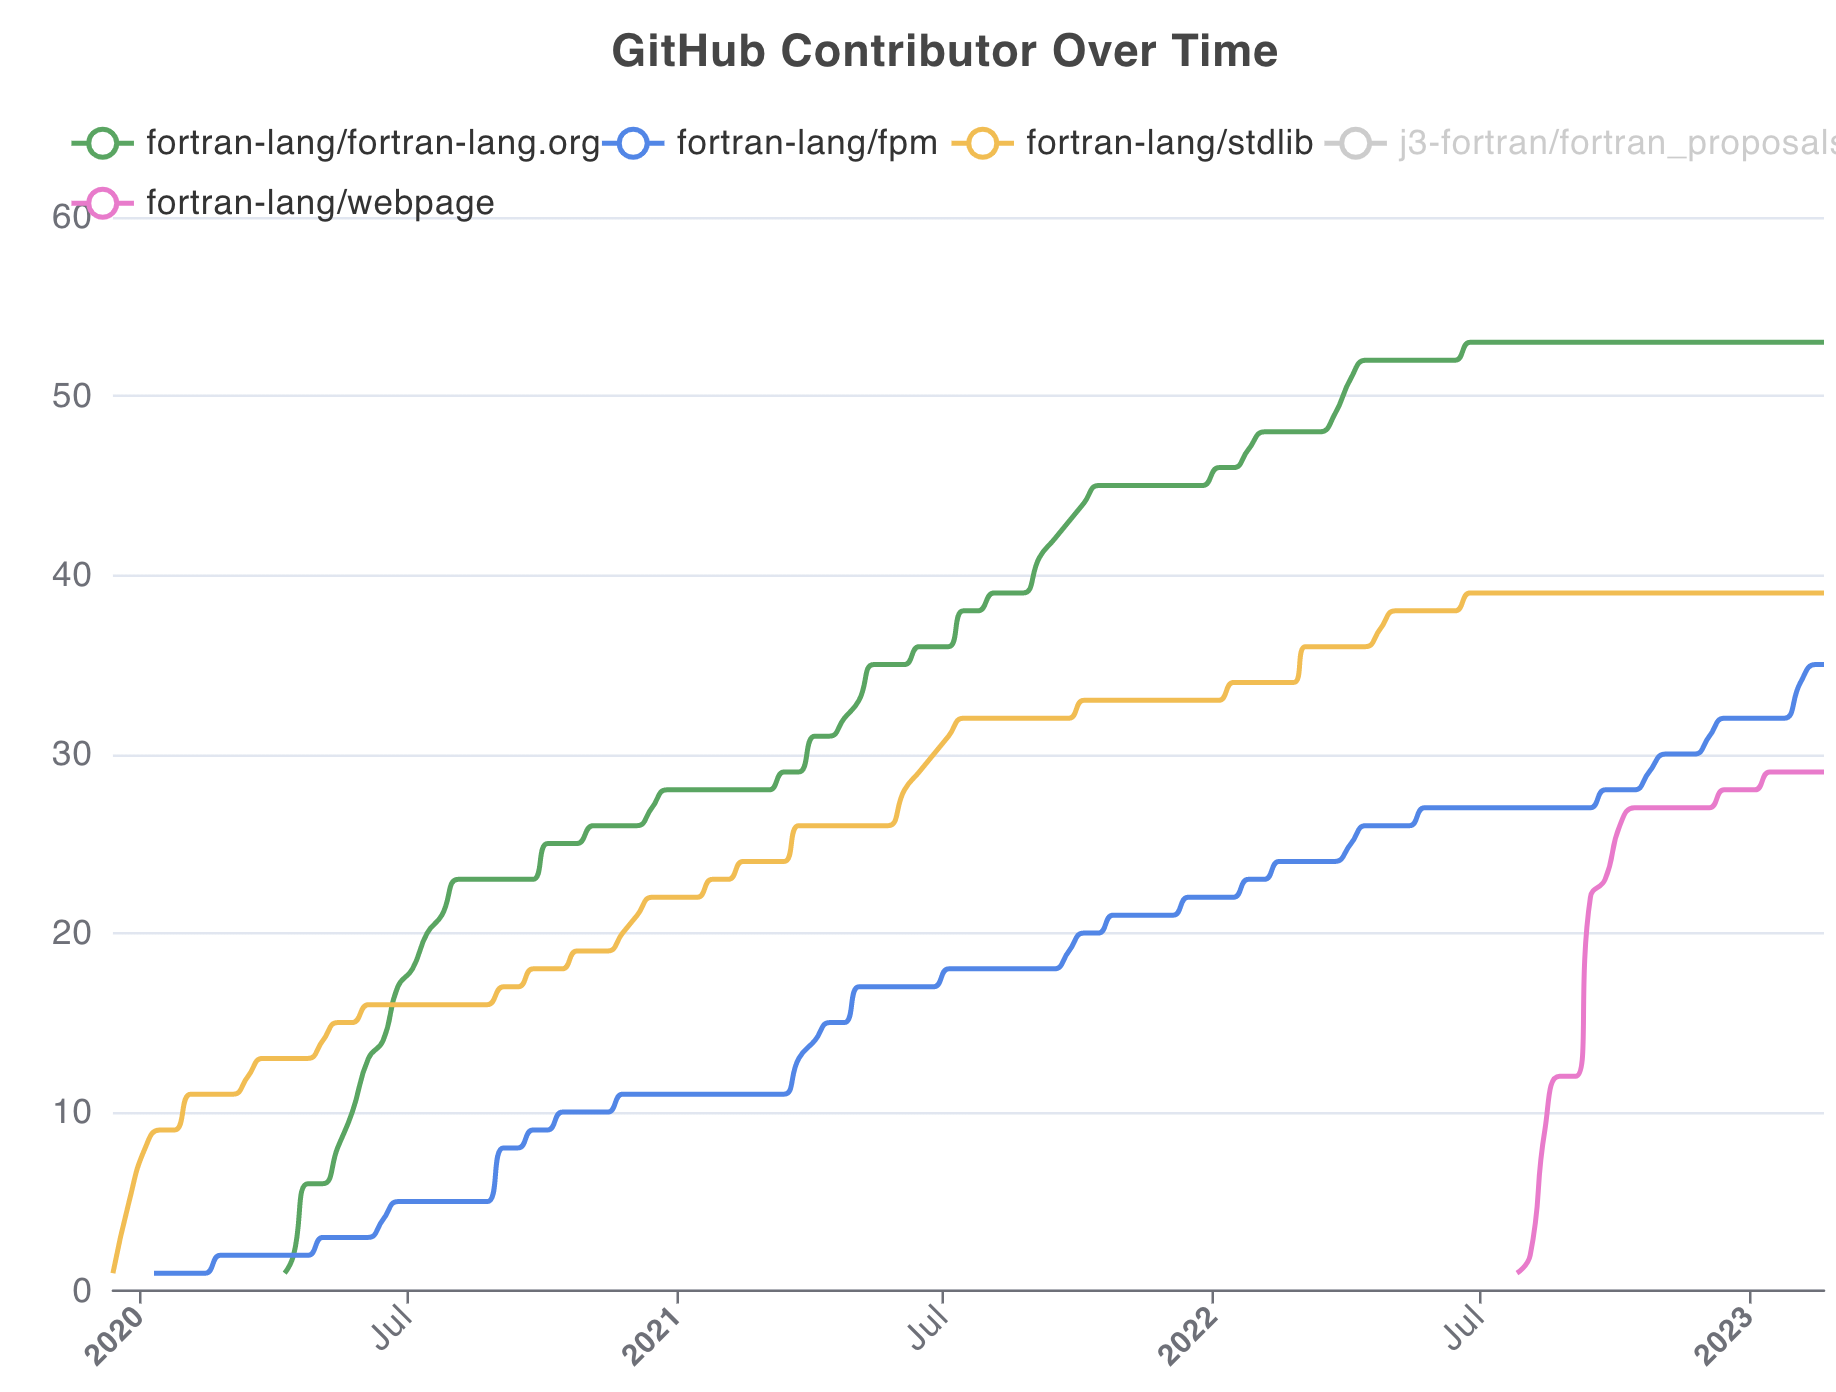
\includegraphics[width=\textwidth]{contributor_graph}
    \caption{Contributor graph}
\end{column}%
\end{columns}

\end{frame}

\begin{frame}{Fortran-lang -- Website}
    \centering
    \begin{figure}
        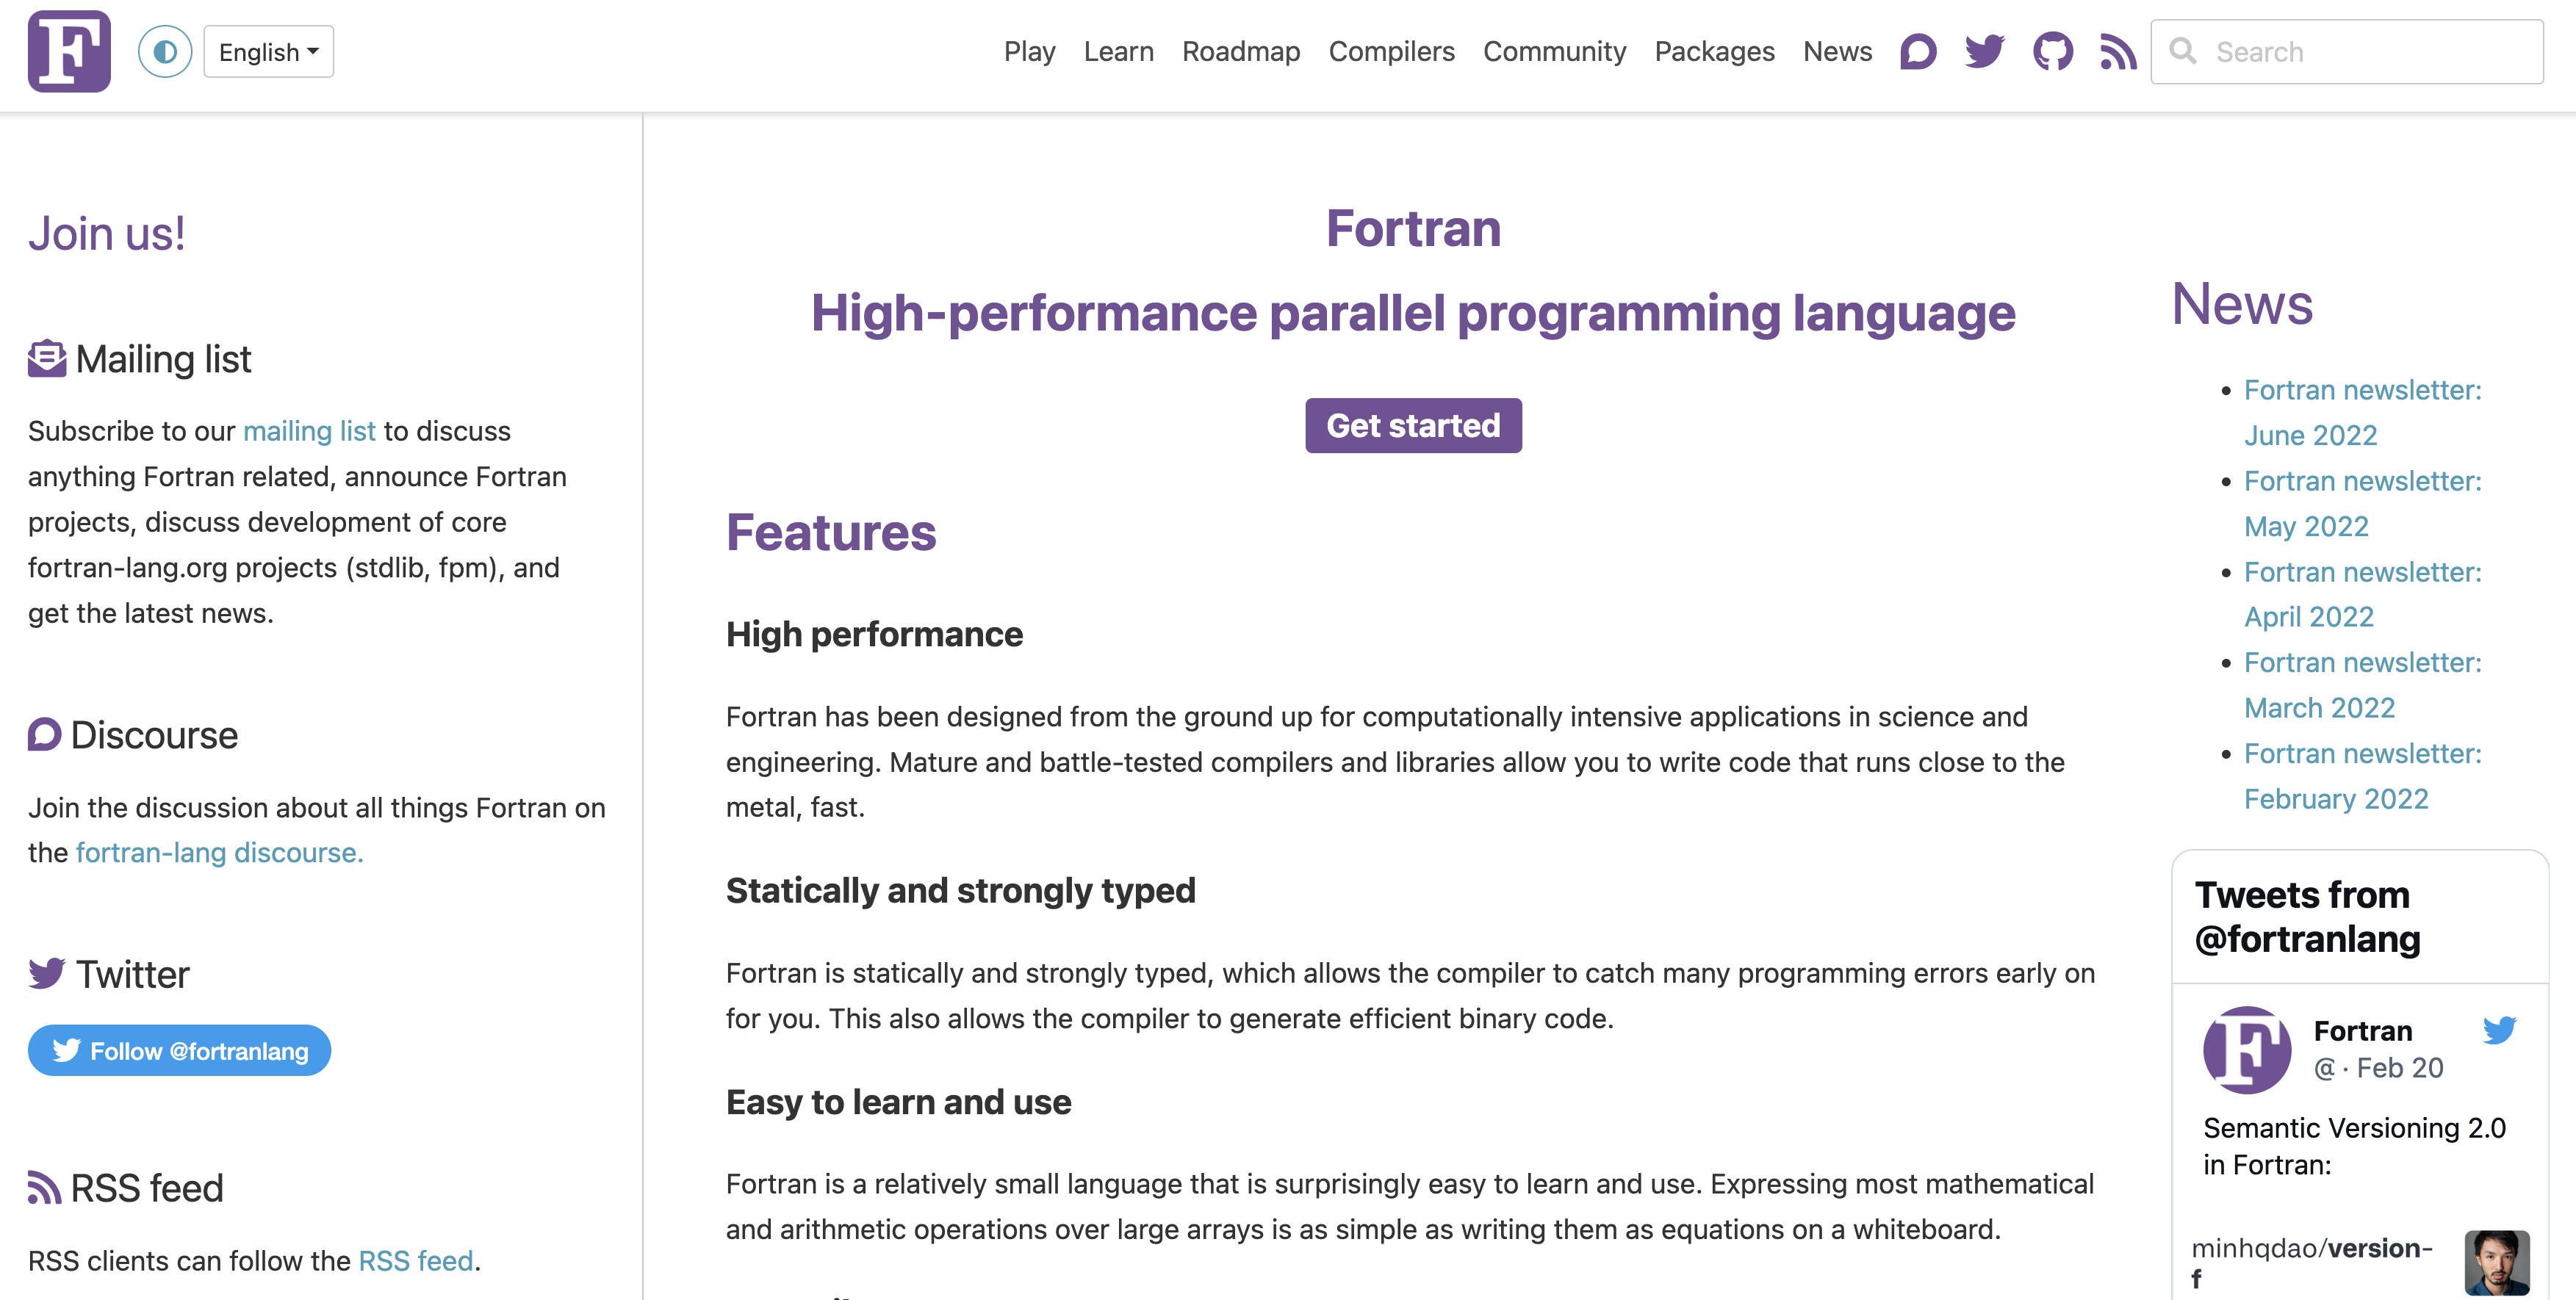
\includegraphics[width=.85\textwidth]{website_screenshot}
    \end{figure}
    \footnotesize\url{https://fortran-lang.org/en/}
\end{frame}

\begin{frame}{Fortran-lang -- Discourse}
\centering
    \begin{figure}
        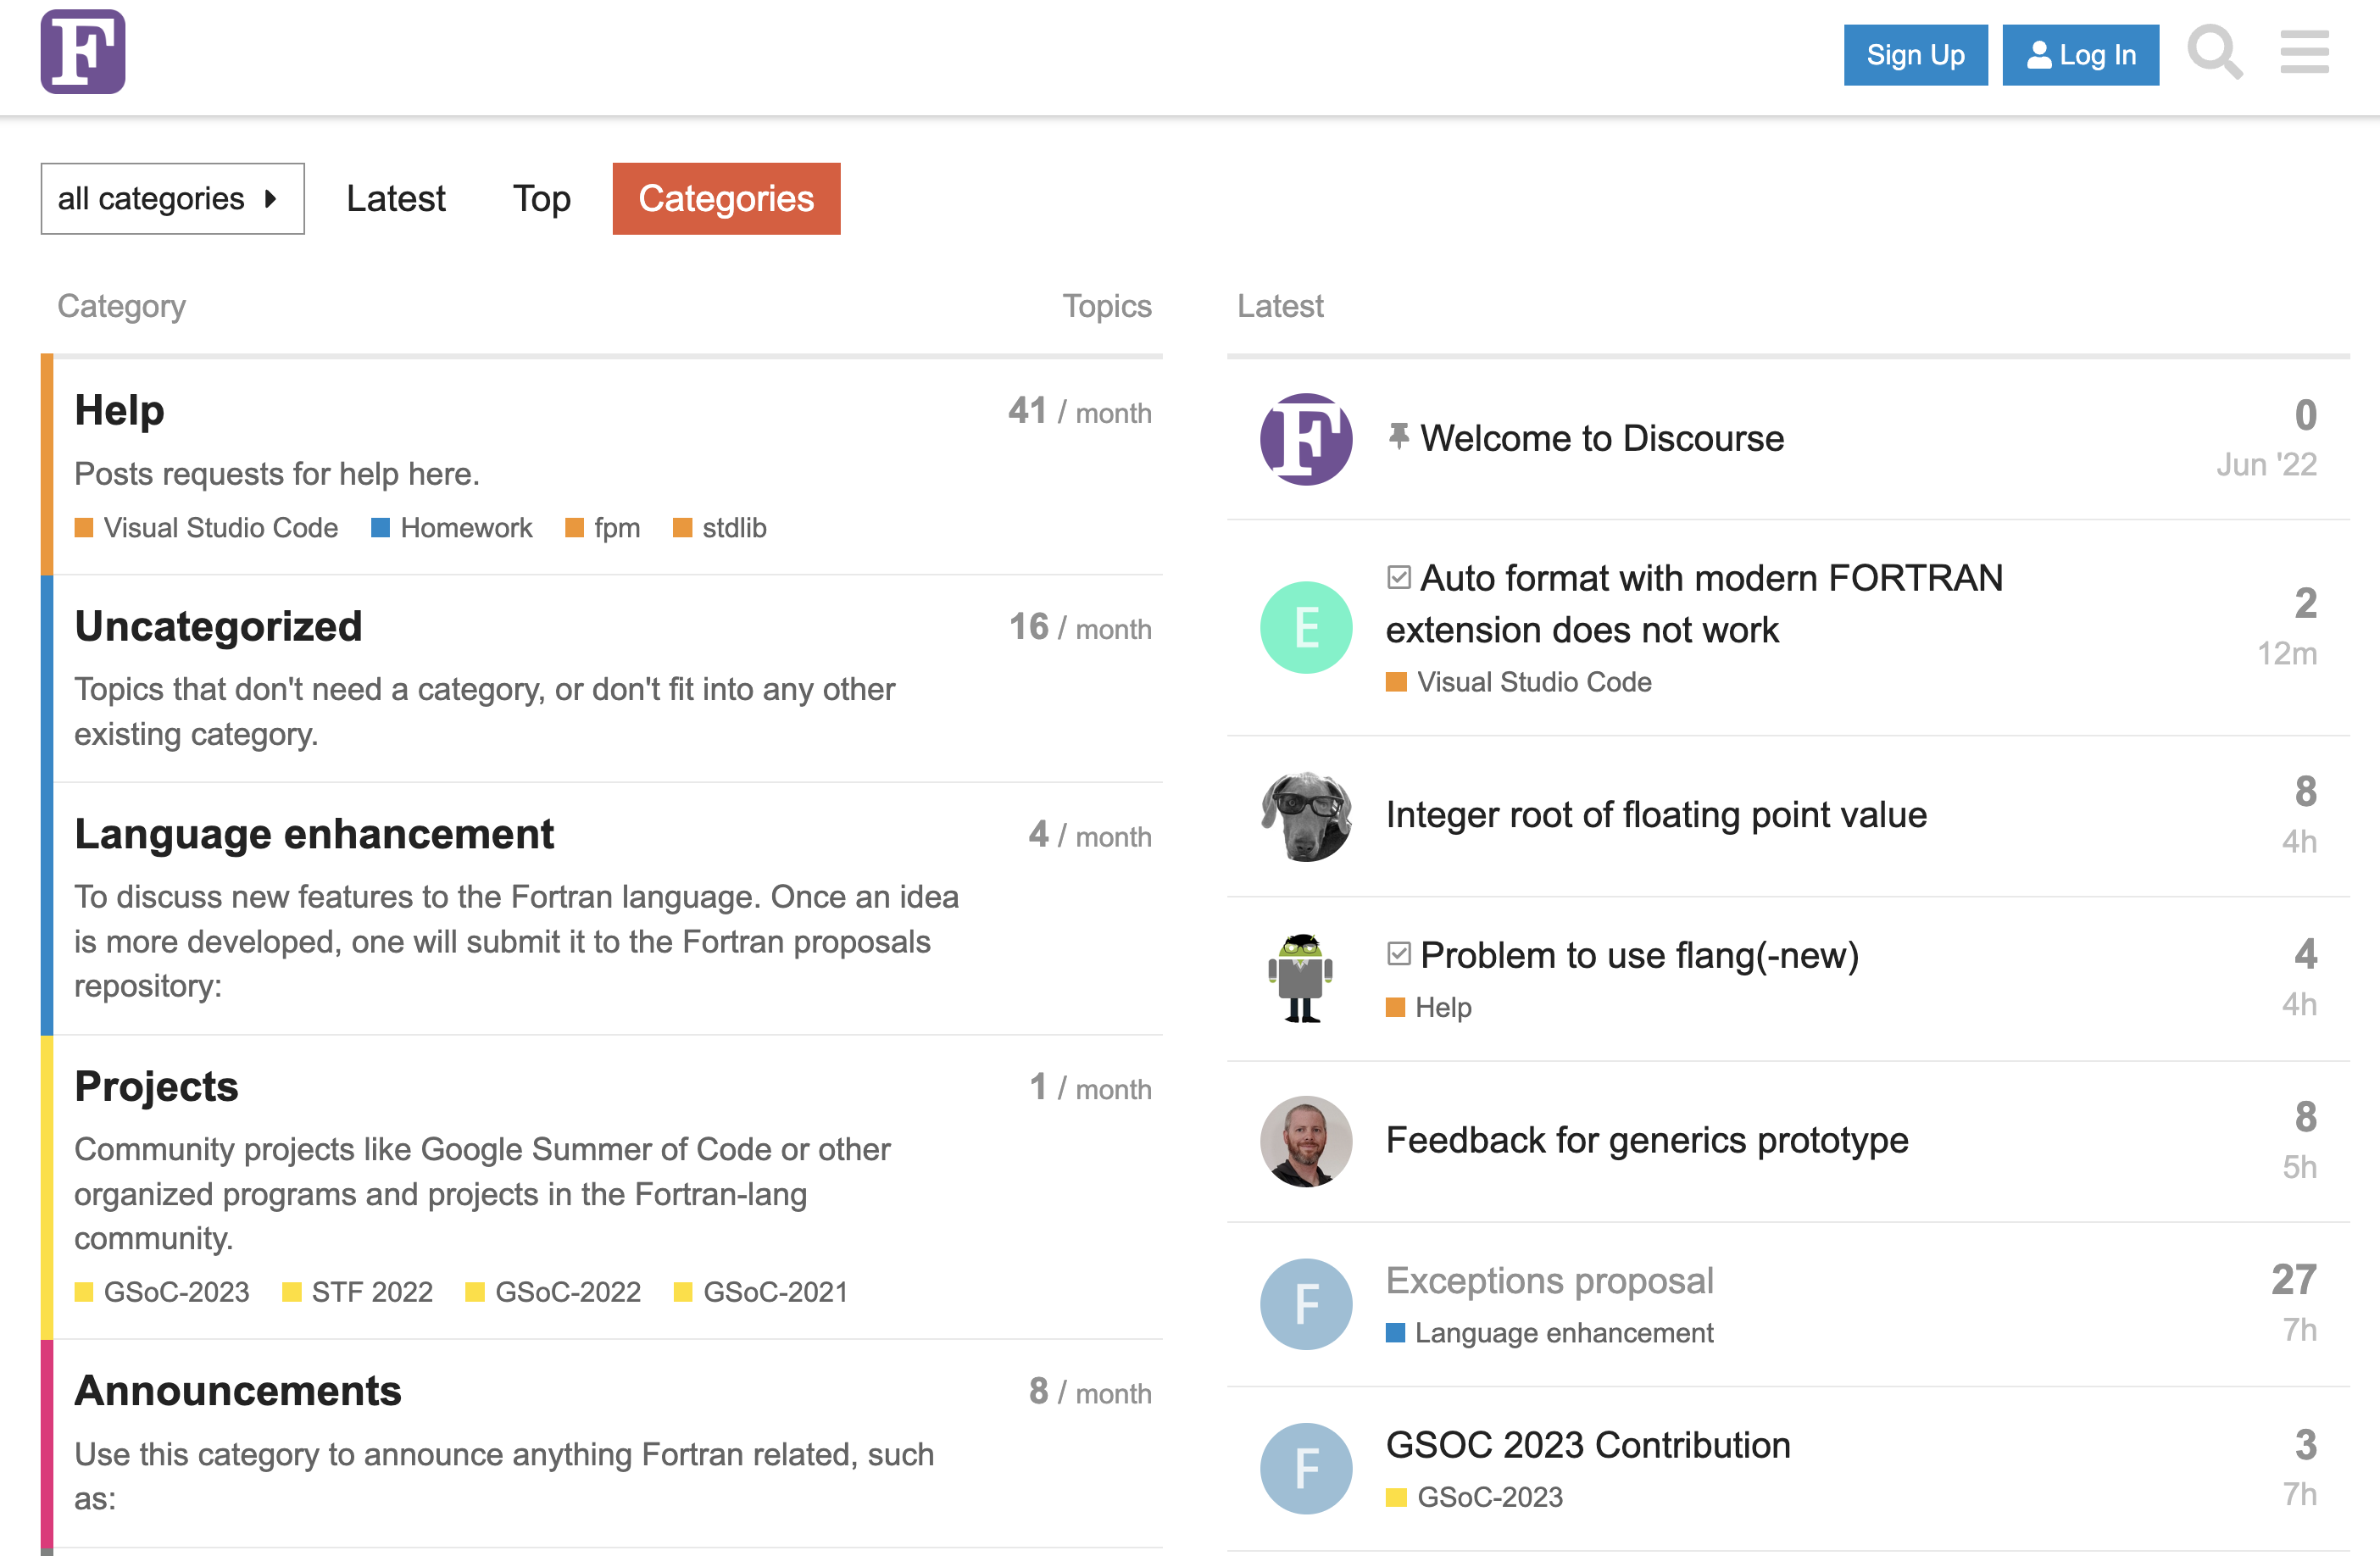
\includegraphics[width=.65\textwidth]{Discourse_screenshot}
    \end{figure}
        \footnotesize\url{https://fortran-lang.discourse.group/}
\end{frame}

\begin{frame}{What about tooling?}
    \centering
    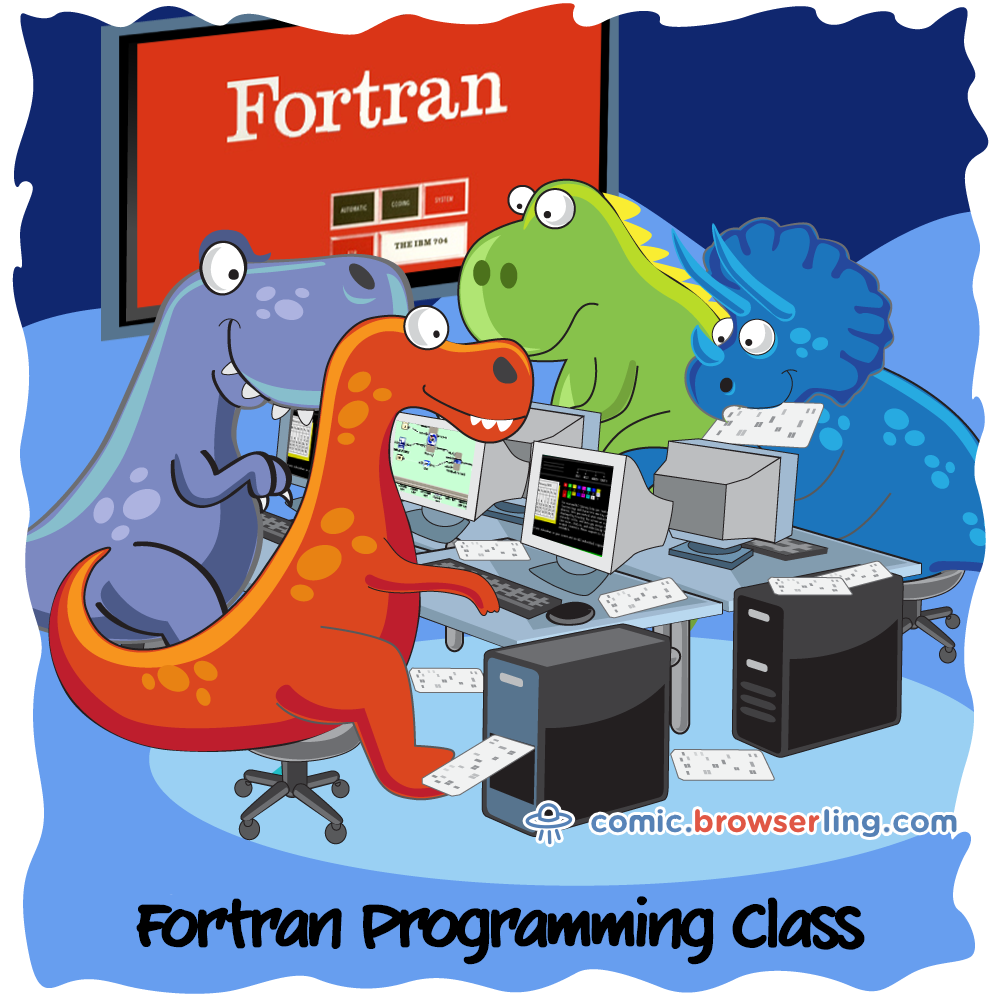
\includegraphics[width=0.4\textwidth]{punch-cards-hires}\\
    \vspace{2mm}\caption{Source: \url{https://comic.browserling.com/49}}
\end{frame}

\begin{frame}
\frametitle{Fortran Package Manager - fpm}
\begin{block}{Aim}
Fortran-specific build system and package manager to ease the learning curve for starting new Fortran projects and composing Fortran software
\end{block}
\begin{itemize}
    \item GitHub: \url{https://github.com/fortran-lang/fpm}
    \item Automatically scans sources for module and submodule dependencies
    \item Incremental and parallel builds
    \item Tree-shaking
    \item fpm is written in Fortran! (Lower the barrier for Fortran users to contribute)
\end{itemize}
\end{frame}


\begin{frame}
\frametitle{Fortran Package Manager - fpm}
    \begin{figure}
        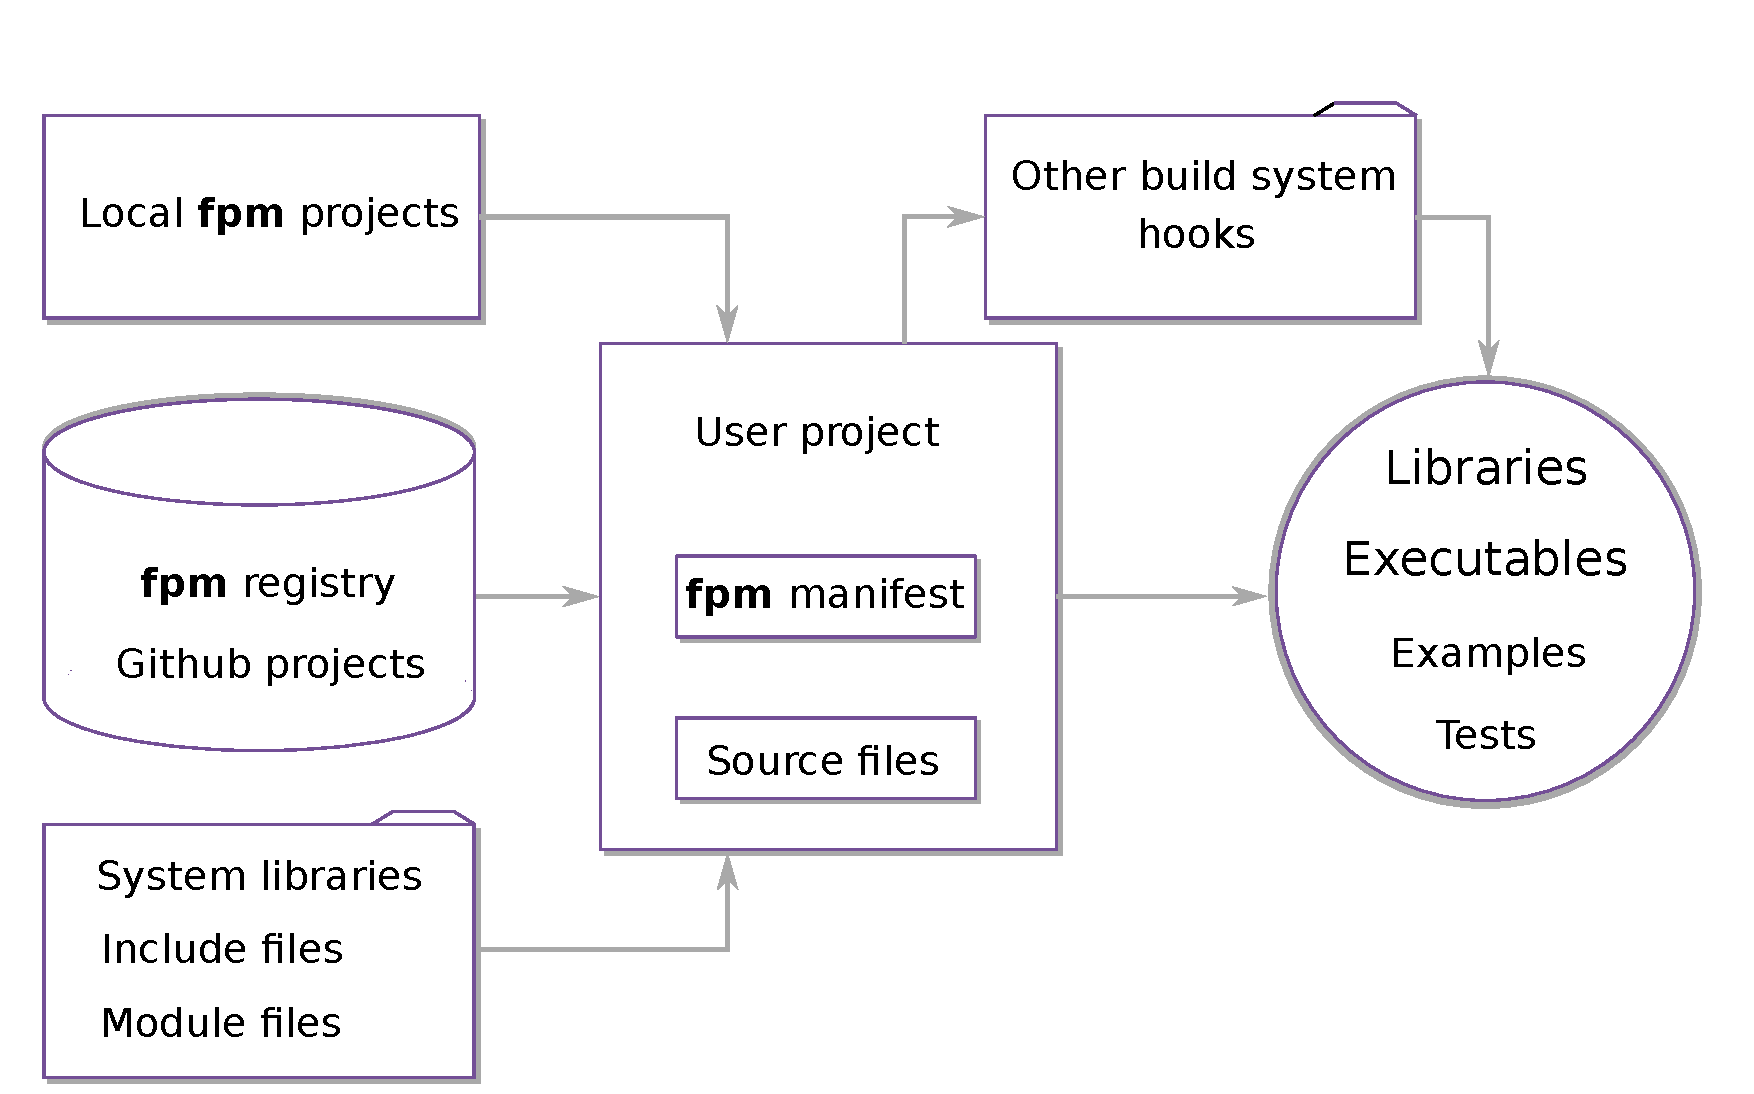
\includegraphics[width=.7\textwidth]{fpm_diagram}\\
        {\footnotesize Source: Kedward, L. J., et al. (2022). The State of Fortran. \textit{CSE}, 24(2), 63-72. \url{https://doi.org/10.1109/MCSE.2022.3159862}}
    \end{figure}
\end{frame}

\begin{frame}{Fortran standard library (\textt{stdlib})}
\begin{block}{Aim}
Develop a community-driven \textit{de facto} standard library for Fortran
\end{block}
\begin{itemize}
    \item GitHub: \url{https://github.com/fortran-lang/stdlib}
    \item Specification: \url{https://stdlib.fortran-lang.org}
\end{itemize}
\begin{block}{Modules}
    \centering
    \begin{tabular}{cccc}
ansi & hashmaps & math & specialfunctions\\
array & io & optval & stats\\
ascii & io\_npy & quadrature & string\_type\\
bitsets & kinds & random & stringlist\_type\\
error & lingalg & selection & strings\\
hash\_\<32,64\>\_bit) & logger & sorting & version
    \end{tabular}
\end{block}
\end{frame}
\begin{frame}
\frametitle{LFortran Compiler}
\begin{columns}[T] % align columns
\begin{column}{.78\textwidth}
{\footnotesize
\begin{itemize}
\item New LLVM-based Community Compiler
\item Also aims to support interactive usage (Jupyter notebooks)
\item Multiple backends (LLVM, x86, C, Julia, WASM, ...)
\item Modular design centred around two modules---AST and ASR
\item Can be used as a library for developing standalone tools
\item Used for prototyping newly suggested language features (generics!)
\end{itemize}}
\begin{itemize}
    \item Website: \url{https://lfortran.org/}
    \item Live playground: \url{https://dev.lfortran.org/}
\end{itemize}
\end{column}%
\hfill%
\begin{column}{.18\textwidth}
    \centering
    
\includegraphics[width=\textwidth]{lfortran_screenshot}
\end{column}%
\end{columns}

\end{frame}

\begin{frame}
\frametitle{Fortran support for Visual Studio Code}
    \begin{figure}
        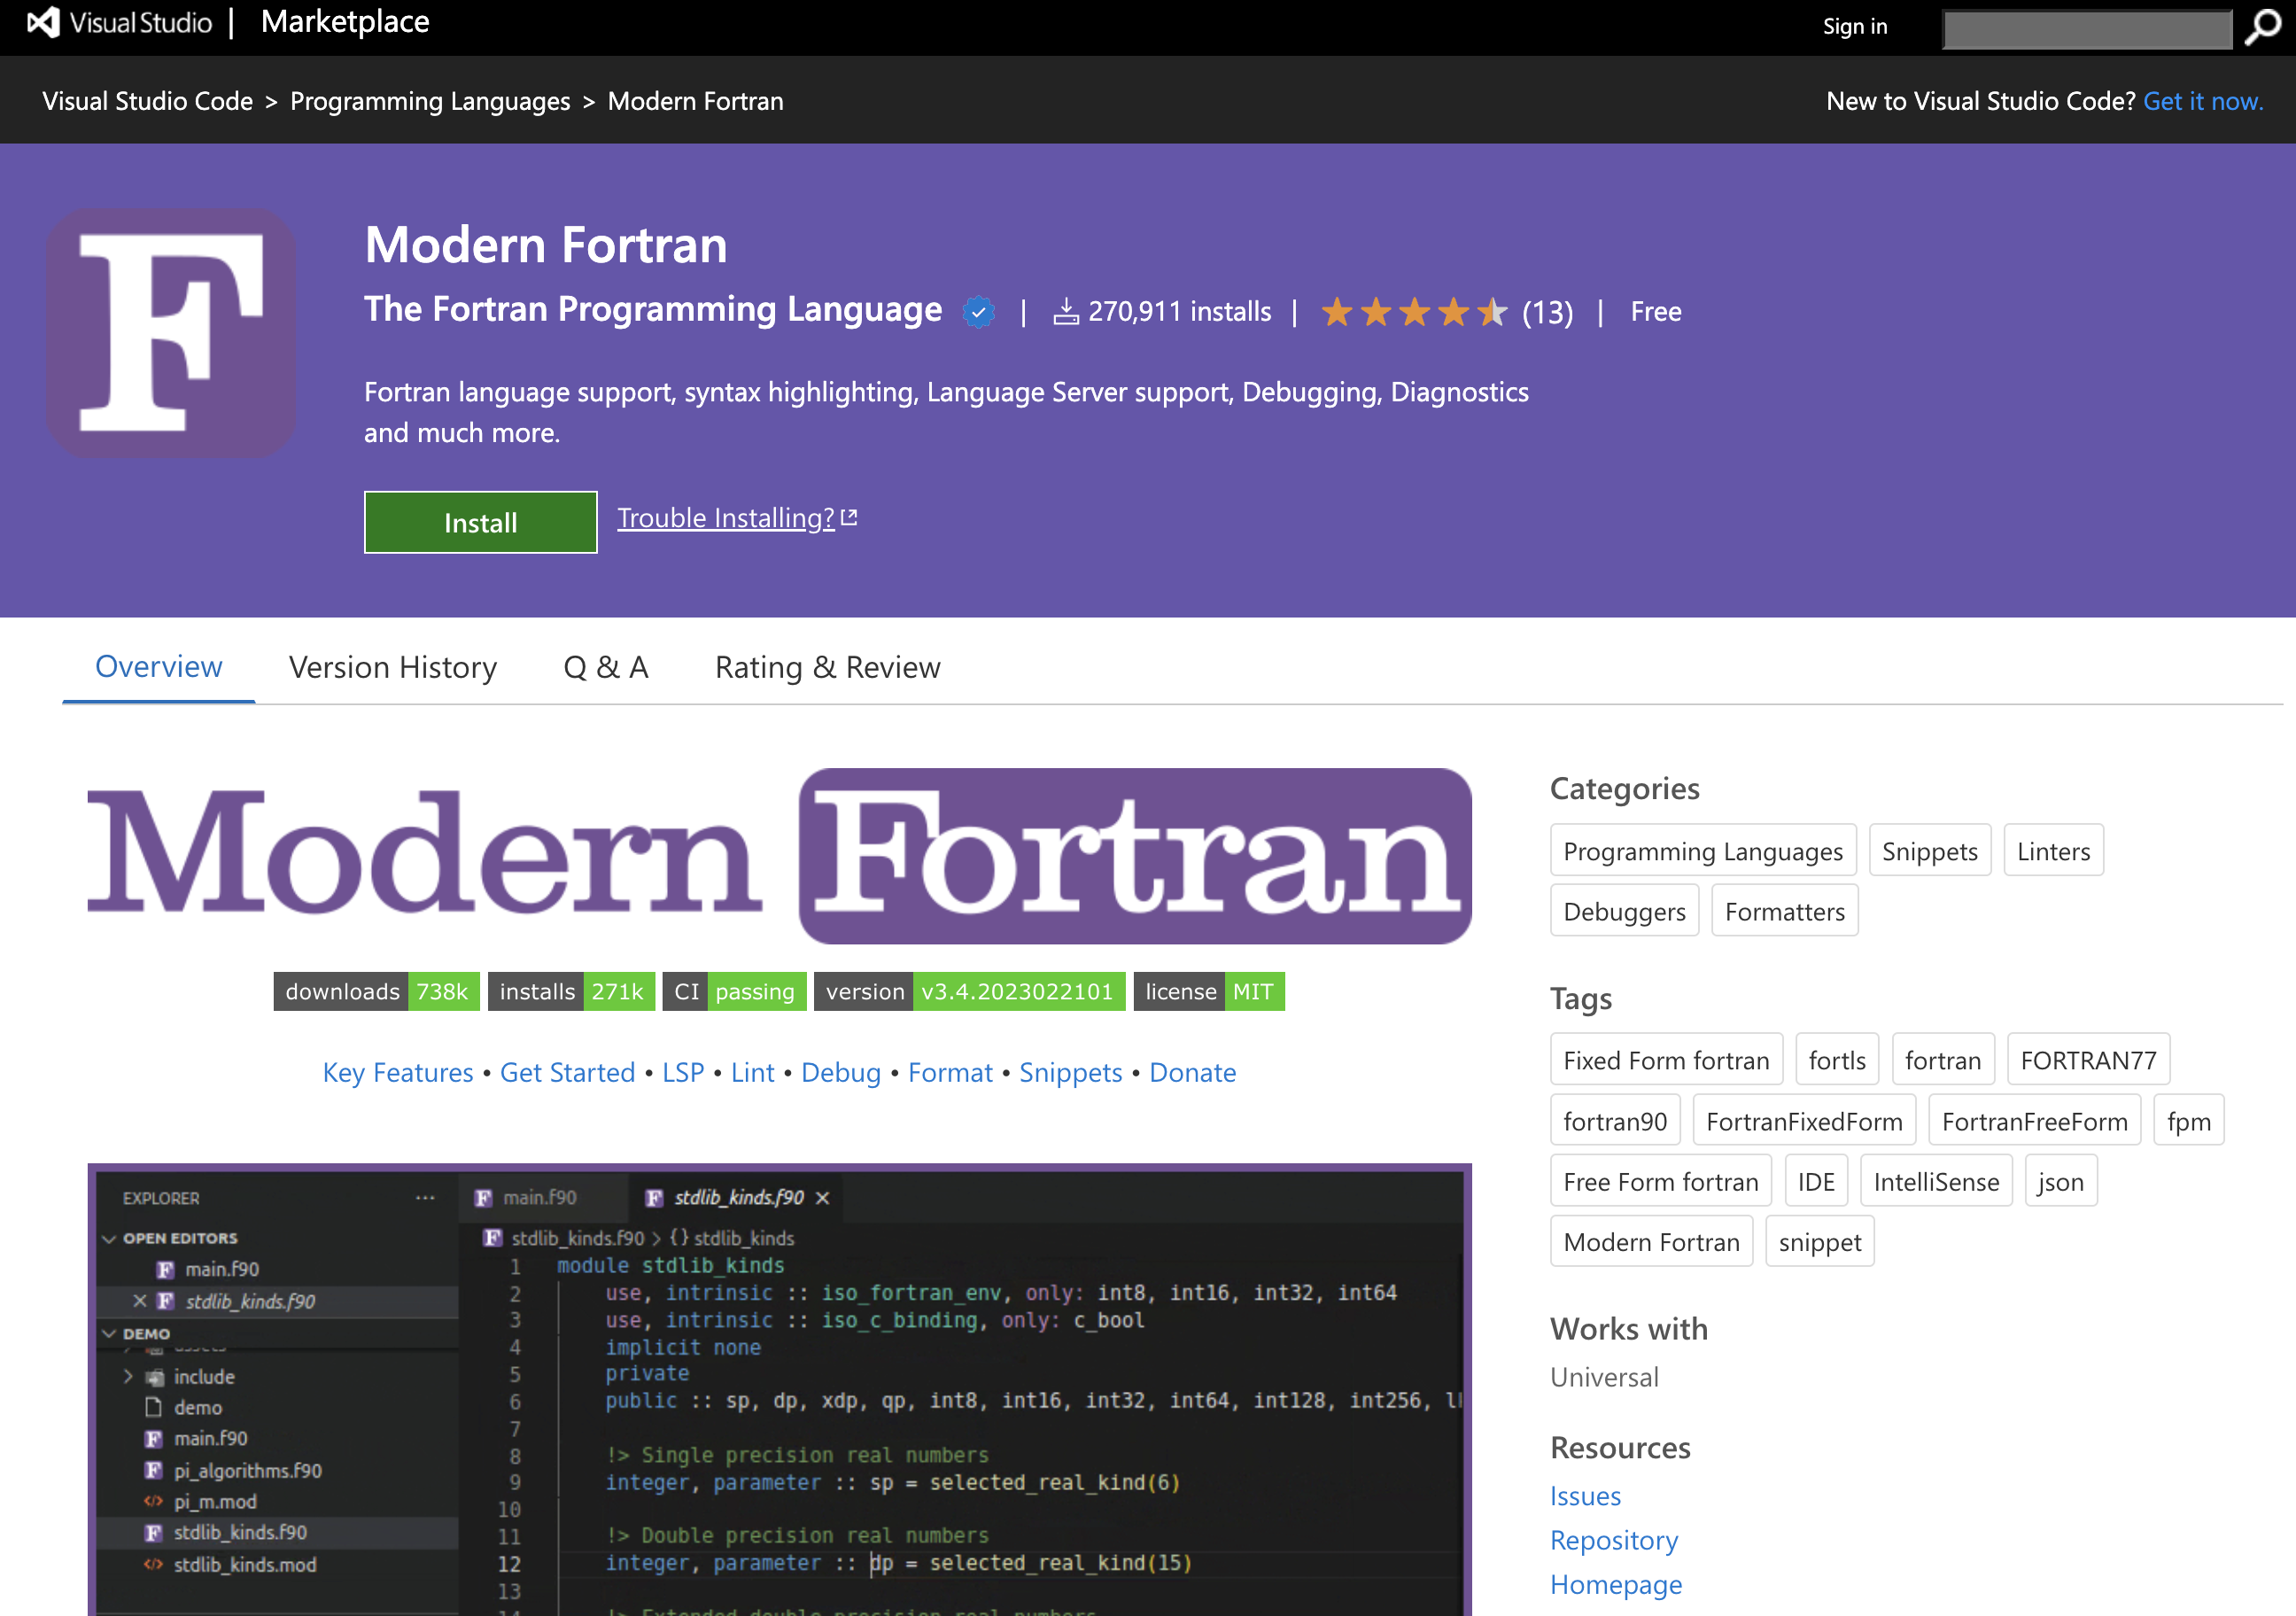
\includegraphics[width=.9\textwidth]{vscode_fortran}
        \url{https://github.com/fortran-lang/vscode-fortran-support}
    \end{figure}
\end{frame}


\begin{frame}{The Future is Bright}
\begin{itemize}
\item Google Summer of Code 2023 (hopefully will be accepted for the third year in a row---announcements today!)
\item Fortran-lang received funding from the Sovereign Tech Fund (\url{https://sovereigntechfund.de/fortran.html})
\begin{itemize}
    \item Fpm package registry
    \item LFortran compiler
\end{itemize}
\item Growing number of fpm packages
\item First ``experiments'' using fpm in Fortran training courses (Universität Bonn, Forschungszentrum Jülich)
\end{itemize}
\end{frame}

\begin{frame}{The End... or a New Beginning?}
    \centering
    
\includegraphics[width=0.8\textwidth]{simpson_horizontal}\\
    \vspace{2mm}
    {\footnotesize Image from u/crazycold15 (Reddit)\\ Originally in Simpsons episode ``The Man Who Came to Be Dinner'' (2015) \\ \url{https://youtu.be/kMQvC03Wx50?t=80}}
\end{frame}

\end{document}
